\documentclass[12pt, a4paper]{article} 

%%%%%%%%%% Математика %%%%%%%%%%
\usepackage{amsmath,amsfonts,amssymb,amsthm,mathtools} 
%%%%%%%%%%%%%%%%%%%%%%%% Шрифты %%%%%%%%%%%%%%%%%%%%%%%%%%%%%%%%%
\usepackage{fontspec}         % пакет для подгрузки шрифтов
\setmainfont{Arial}   % задаёт основной шрифт документа

\defaultfontfeatures{Mapping=tex-text}
\usepackage{unicode-math}     % пакет для установки математического шрифта
\setmathfont{Asana Math}      % шрифт для математики

\usepackage{polyglossia}      % Пакет, который позволяет подгружать русские буквы
\setdefaultlanguage{russian}  % Основной язык документа
\setotherlanguage{english}    % Второстепенный язык документа

%%%%%%%%%% Работа с картинками %%%%%%%%%
\usepackage{graphicx}                  % Для вставки рисунков
\usepackage{graphics} 
\graphicspath{{pop-art/}{pictures/}}    % можно указать папки с картинками
\usepackage{wrapfig}                   % Обтекание рисунков и таблиц текстом
\usepackage{subfigure}                 % для создания нескольких рисунков
\begin{document}

\begin{figure}[h!]

\begin{minipage}[h!]{0.3\linewidth} 
% Обратите внимание на \linewidth-длину текста в теущем окружении!
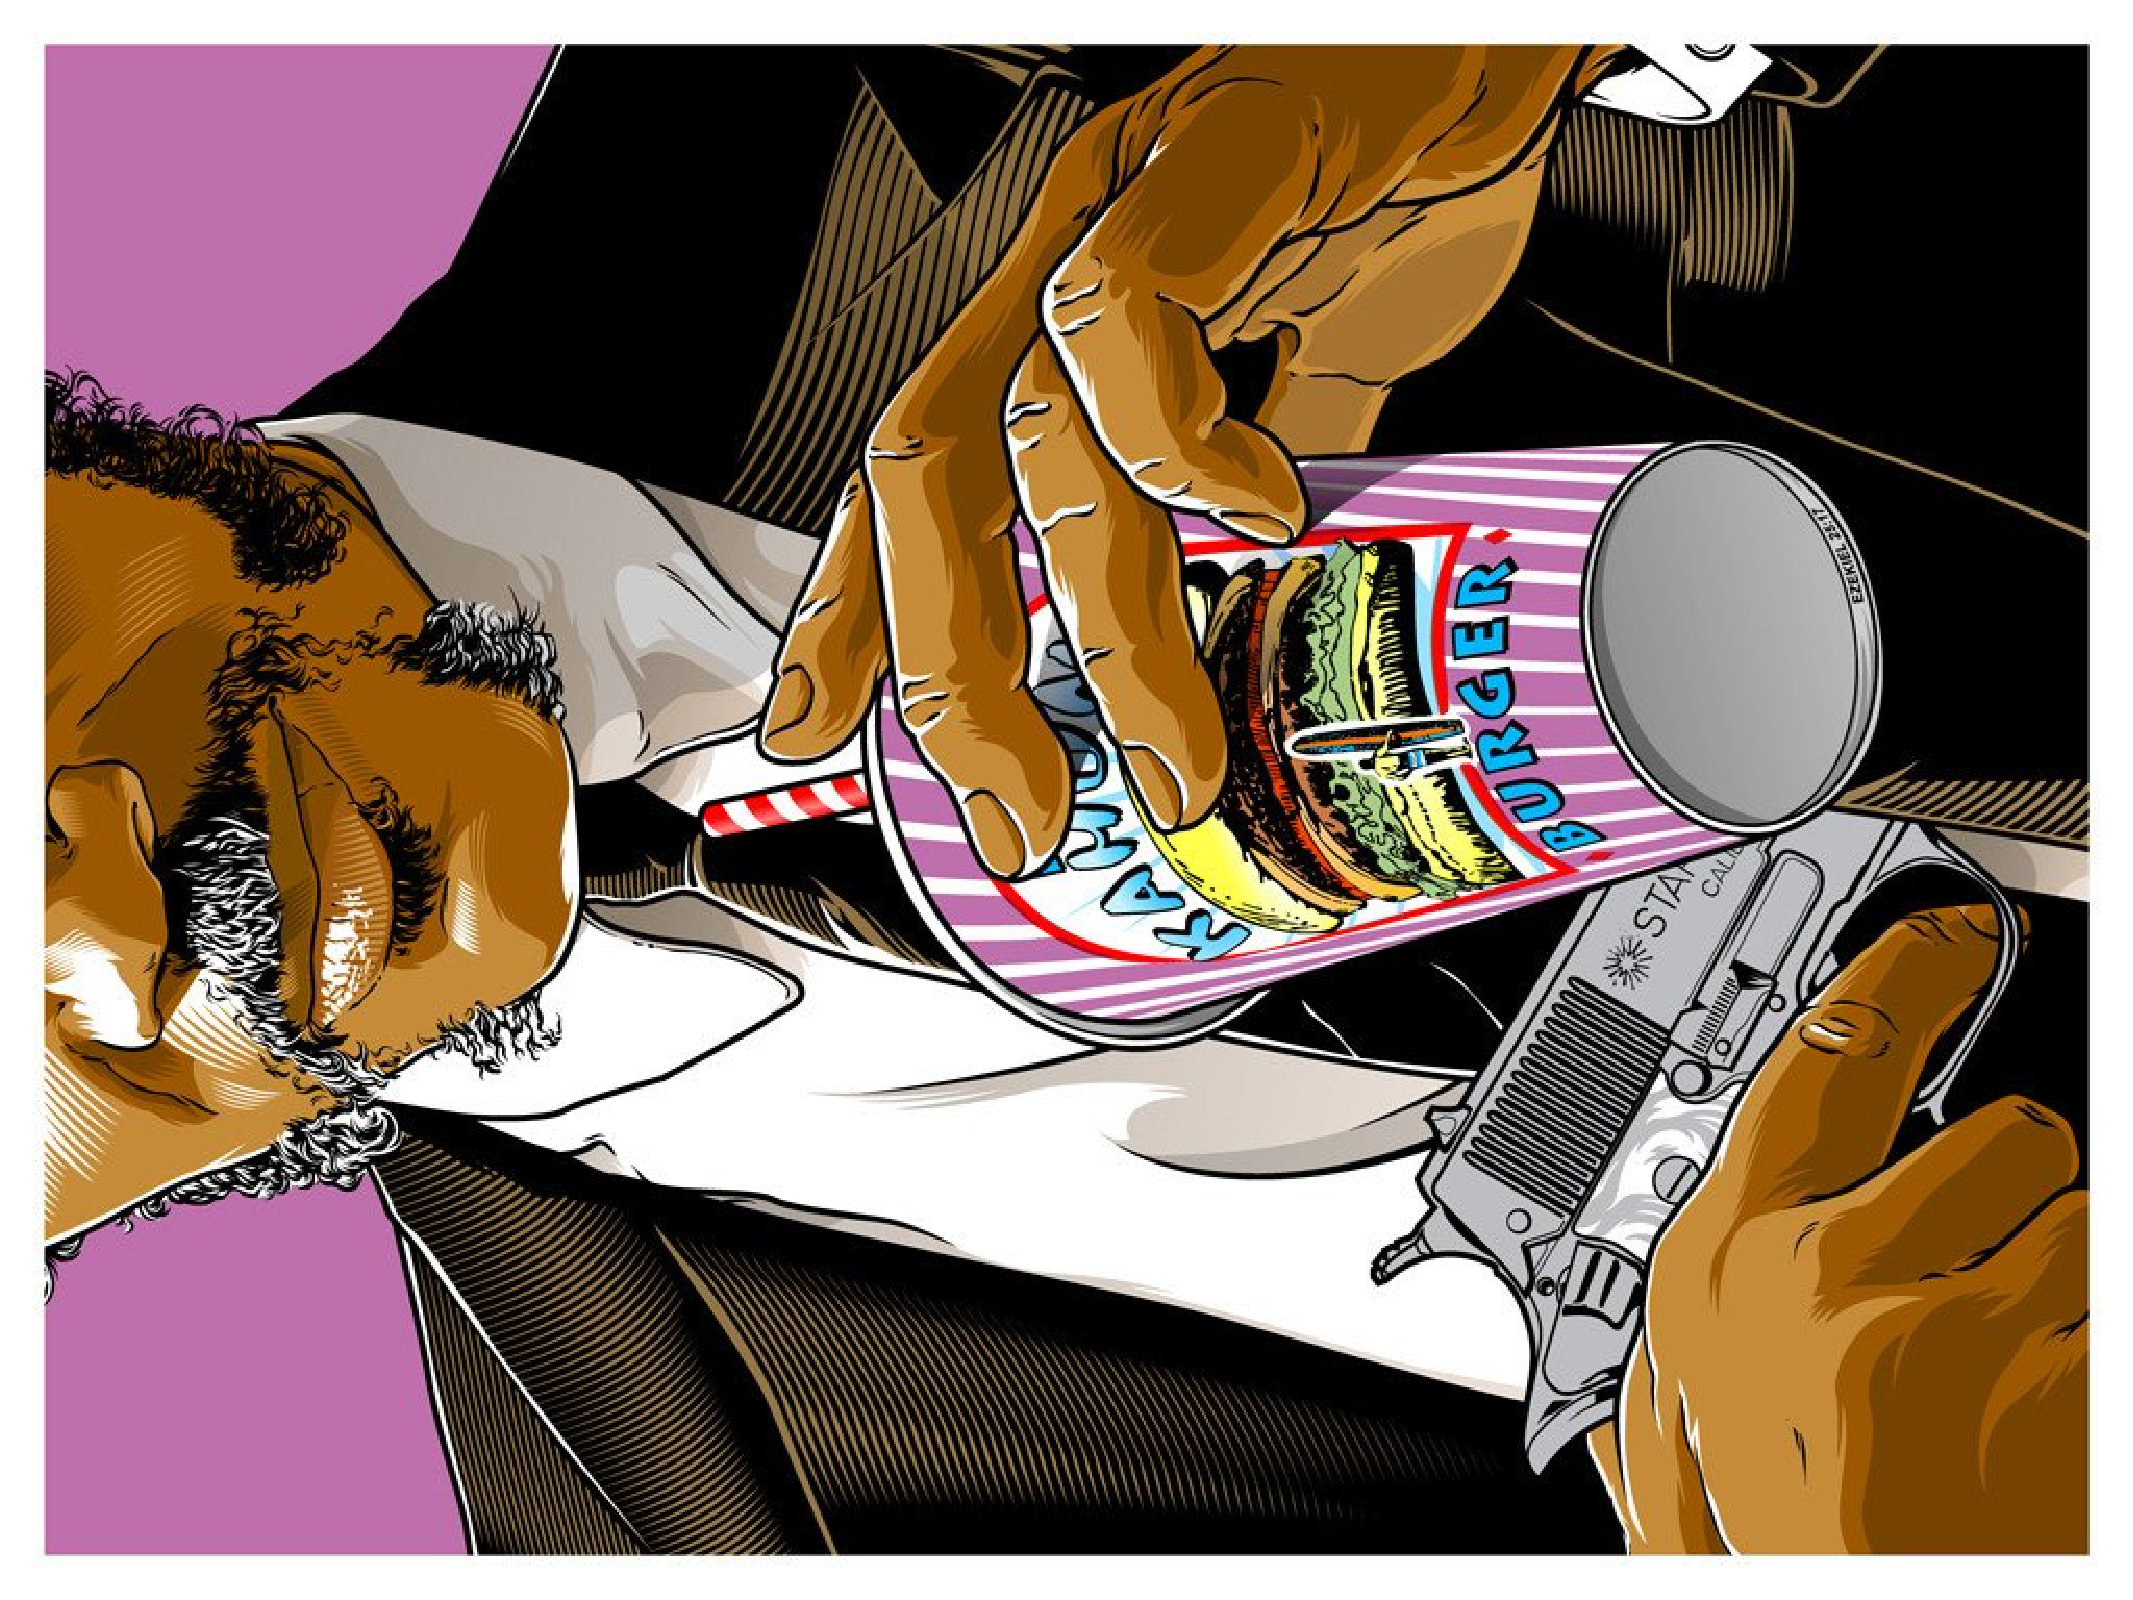
\includegraphics[height=4cm,width=6cm,keepaspectratio,scale=0.15,angle=270]{pop1.pdf}
\end{minipage}
\hfill
\begin{minipage}[h!]{0.3\linewidth}
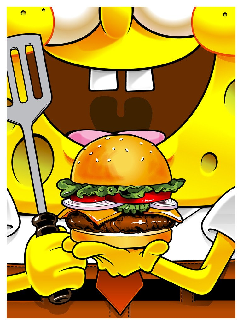
\includegraphics[scale=0.975]{pop8.pdf}
\end{minipage}
\hfill
\begin{minipage}[h!]{0.3\linewidth}

\includegraphics[scale=14.855]{pop3.pdf}
\end{minipage}
\hfill
\begin{minipage}[h!]{0.3\linewidth}
\includegraphics[scale=0.0148]{pop5.pdf}
\end{minipage}
\hfill
\begin{minipage}[h!]{0.3\linewidth}
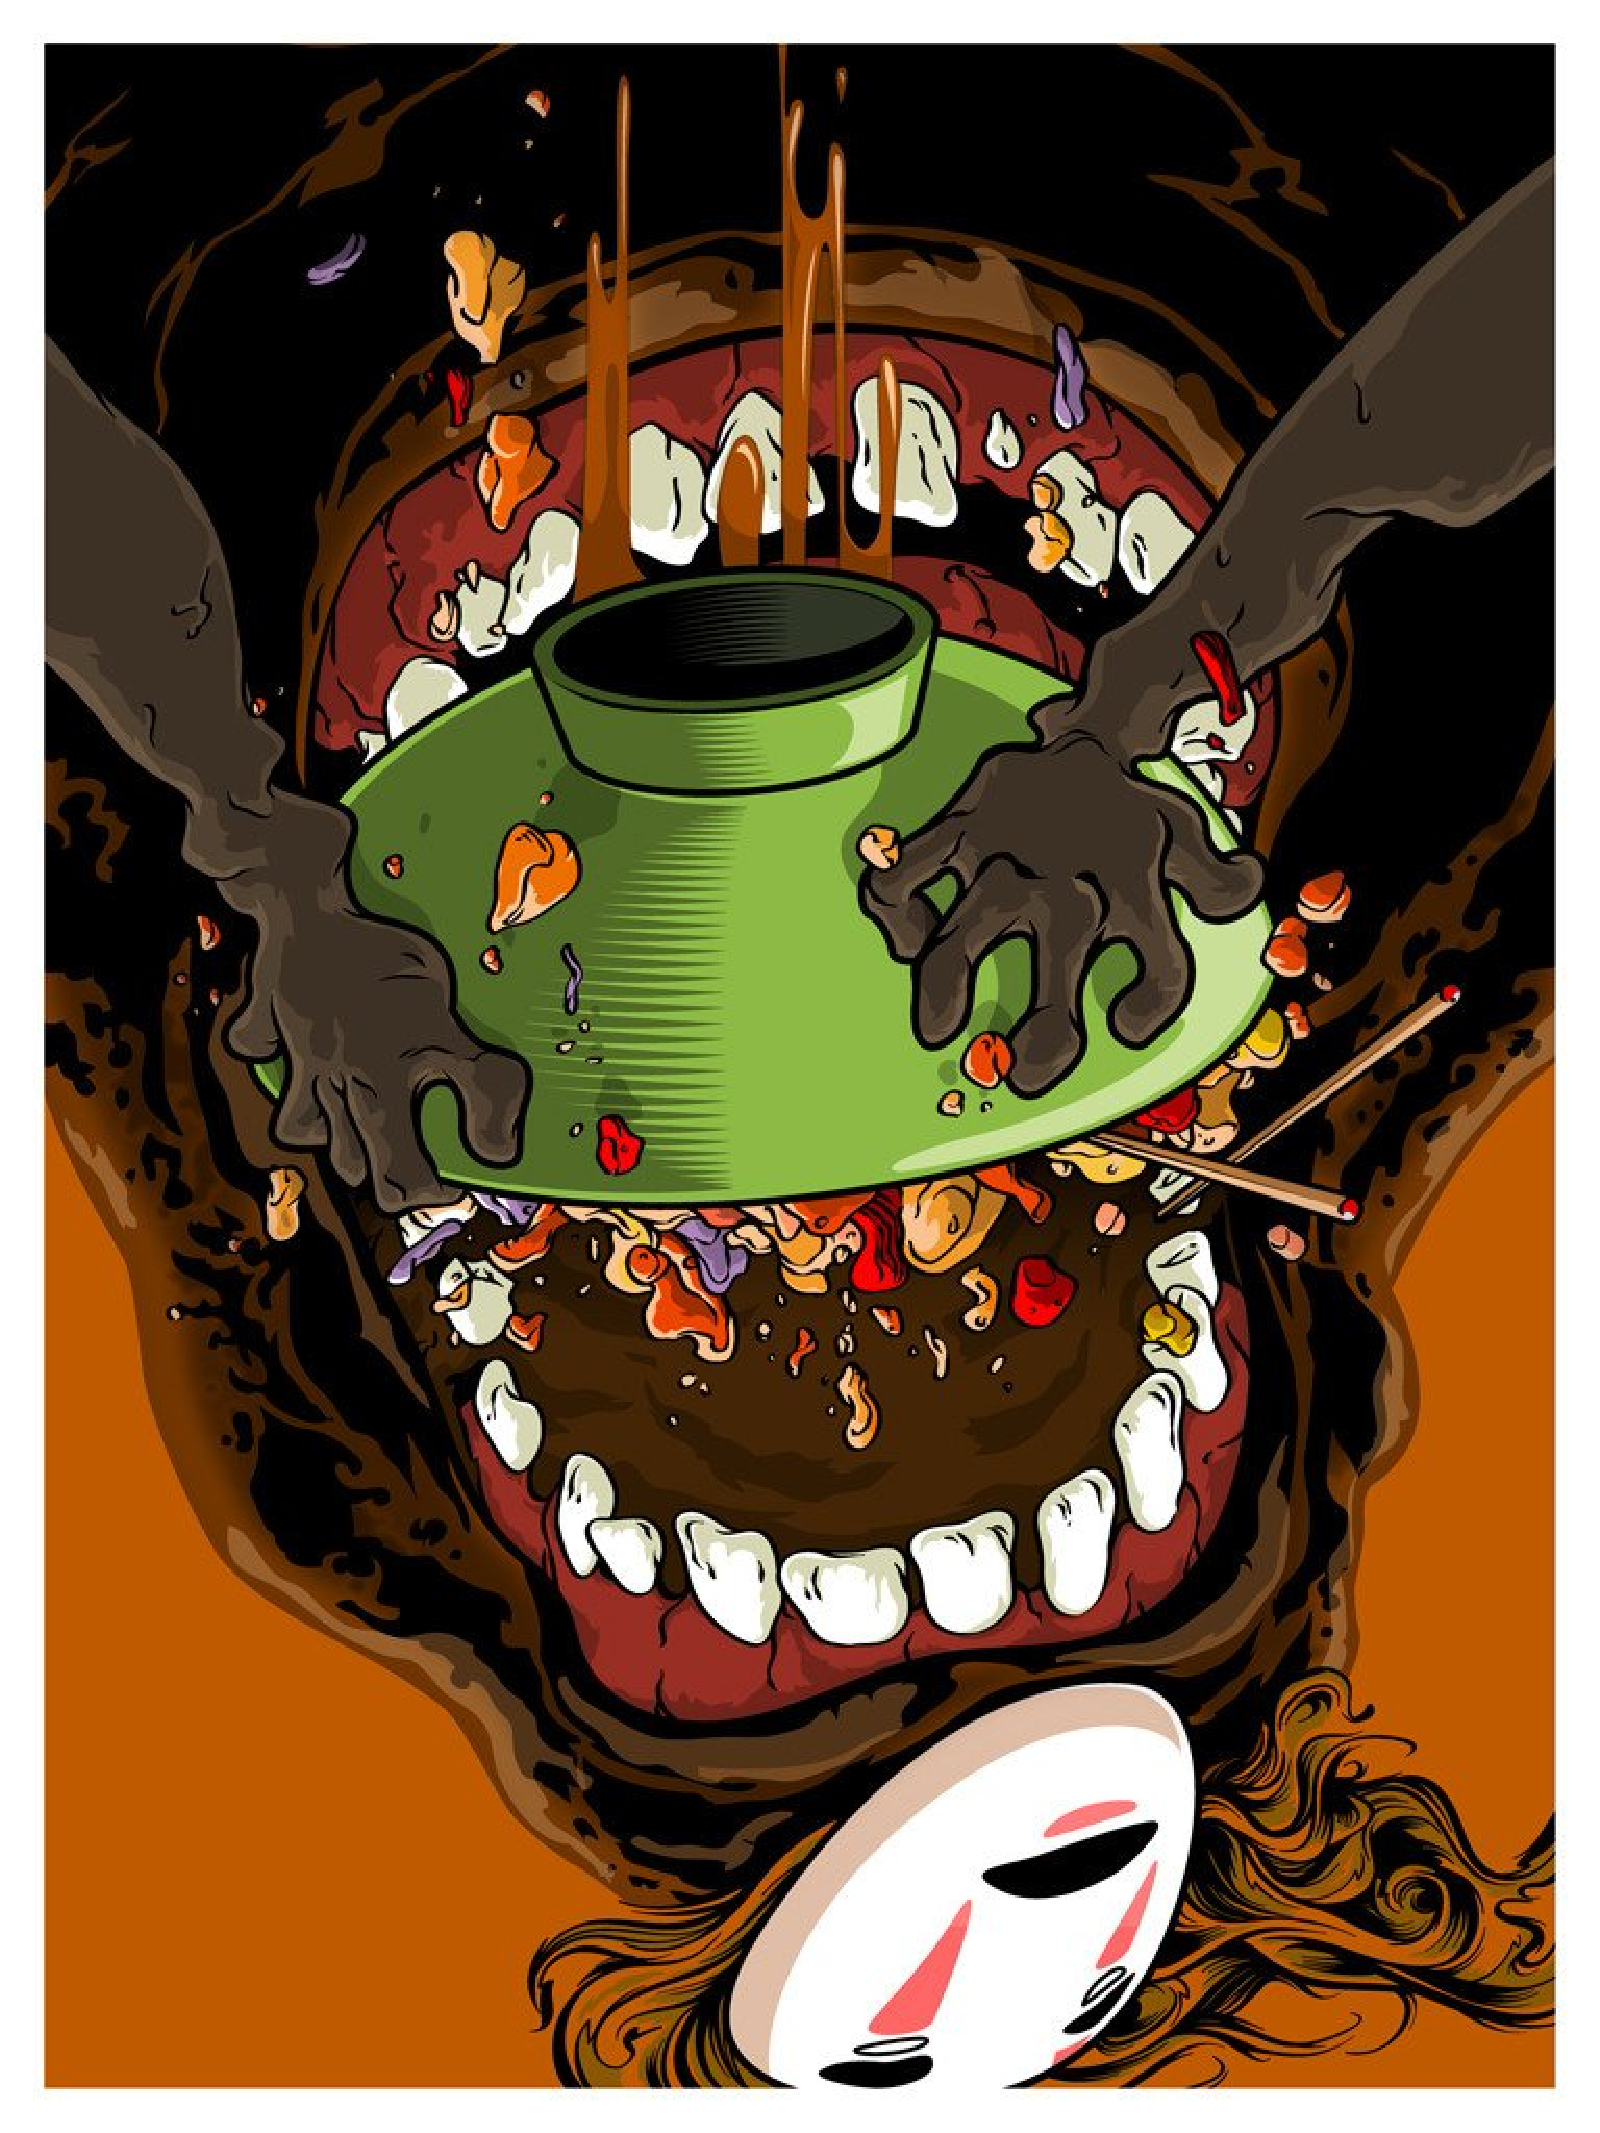
\includegraphics[scale=0.15,angle=180]{pop6.pdf}
\end{minipage}
\hfill
\begin{minipage}[h!]{0.3\linewidth}
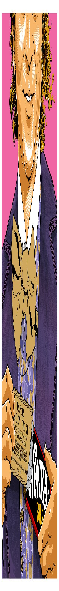
\includegraphics[scale=2,width=4cm,height=5.5cm]{pop7.pdf}
\end{minipage}
\caption{Это что, поп арт?}
\label{fig:1figs}
\end{figure}




\end{document}
